\section{Results}\label{sec:results}

\subsection{Few-Shot Detection}\label{sec:res-fewshot}
Table~\ref{tab:k10} lists all metrics at the default $k=10$; the complete curves for $k=1\ldots$all are in the repository. \emph{PatchCore-lite is the most accurate detector at every $k$}: averaged over the five textures its image AUROC is 0.904 with a single shot, 0.916 at $k=10$, and 0.977 with the full training set (AUPRO 0.747, 0.786, 0.894). \emph{The stationary Gabor--Gaussian model is the most shot-efficient}: it reaches 0.828 at $k=1$---better than PaDiM (0.725), whose per-position Gaussians are poorly estimated from few images---and saturates early (0.860 at $k=10$, 0.872 with all shots). The gap between station and edge model is \emph{fabric-dependent}: on leather, tile, and wood the station model is within 0.07 AUROC of PatchCore-lite, whereas on carpet (0.740 vs.\ 0.967) and grid (0.674 vs.\ 0.636) it is not adequate at $k=10$. Grid is hard for all detectors with few shots and improves with more normal data (PatchCore-lite 0.921 with all 264 images).

Fig.~\ref{fig:qual} shows typical anomaly maps. Both models localise the carpet thread, the leather cut, and the tile crack, and both miss the small broken cells of the grid. On wood the colour-sensitive station model flags the bleached scratch whereas PatchCore-lite stays below its threshold: the models are complementary rather than nested. This fabric dependence motivates the two-tier design.

\begin{table*}[t]
\centering
\caption{Detection and localisation with $k=10$ defect-free shots (mean of three random draws). GG: Gabor--Gaussian (station), PC: PatchCore-lite (edge), PD: PaDiM. Best per metric in bold.}
\label{tab:k10}
\footnotesize
\begin{tabular}{@{}lccccccccc@{}}
\toprule
& \multicolumn{3}{c}{Image AUROC} & \multicolumn{3}{c}{Pixel AUROC} & \multicolumn{3}{c}{AUPRO} \\
\cmidrule(lr){2-4}\cmidrule(lr){5-7}\cmidrule(l){8-10}
Category & GG & PC & PD & GG & PC & PD & GG & PC & PD \\
\midrule
carpet & 0.740 & \textbf{0.967} & 0.881 & 0.883 & \textbf{0.988} & 0.972 & 0.643 & \textbf{0.933} & 0.911 \\
grid & \textbf{0.674} & 0.636 & 0.633 & 0.621 & \textbf{0.742} & 0.676 & 0.178 & \textbf{0.333} & 0.330 \\
leather & 0.984 & \textbf{0.999} & 0.961 & \textbf{0.993} & 0.992 & 0.989 & \textbf{0.984} & 0.965 & 0.967 \\
tile & 0.919 & \textbf{0.986} & 0.841 & 0.936 & \textbf{0.940} & 0.820 & 0.768 & \textbf{0.817} & 0.606 \\
wood & 0.981 & \textbf{0.992} & 0.989 & \textbf{0.932} & 0.929 & 0.931 & 0.879 & 0.882 & \textbf{0.908} \\ \midrule
\textit{Mean} & 0.860 & \textbf{0.916} & 0.861 & 0.873 & \textbf{0.918} & 0.878 & 0.690 & \textbf{0.786} & 0.744 \\
\bottomrule
\end{tabular}
\end{table*}


\begin{figure}[t]
\centering
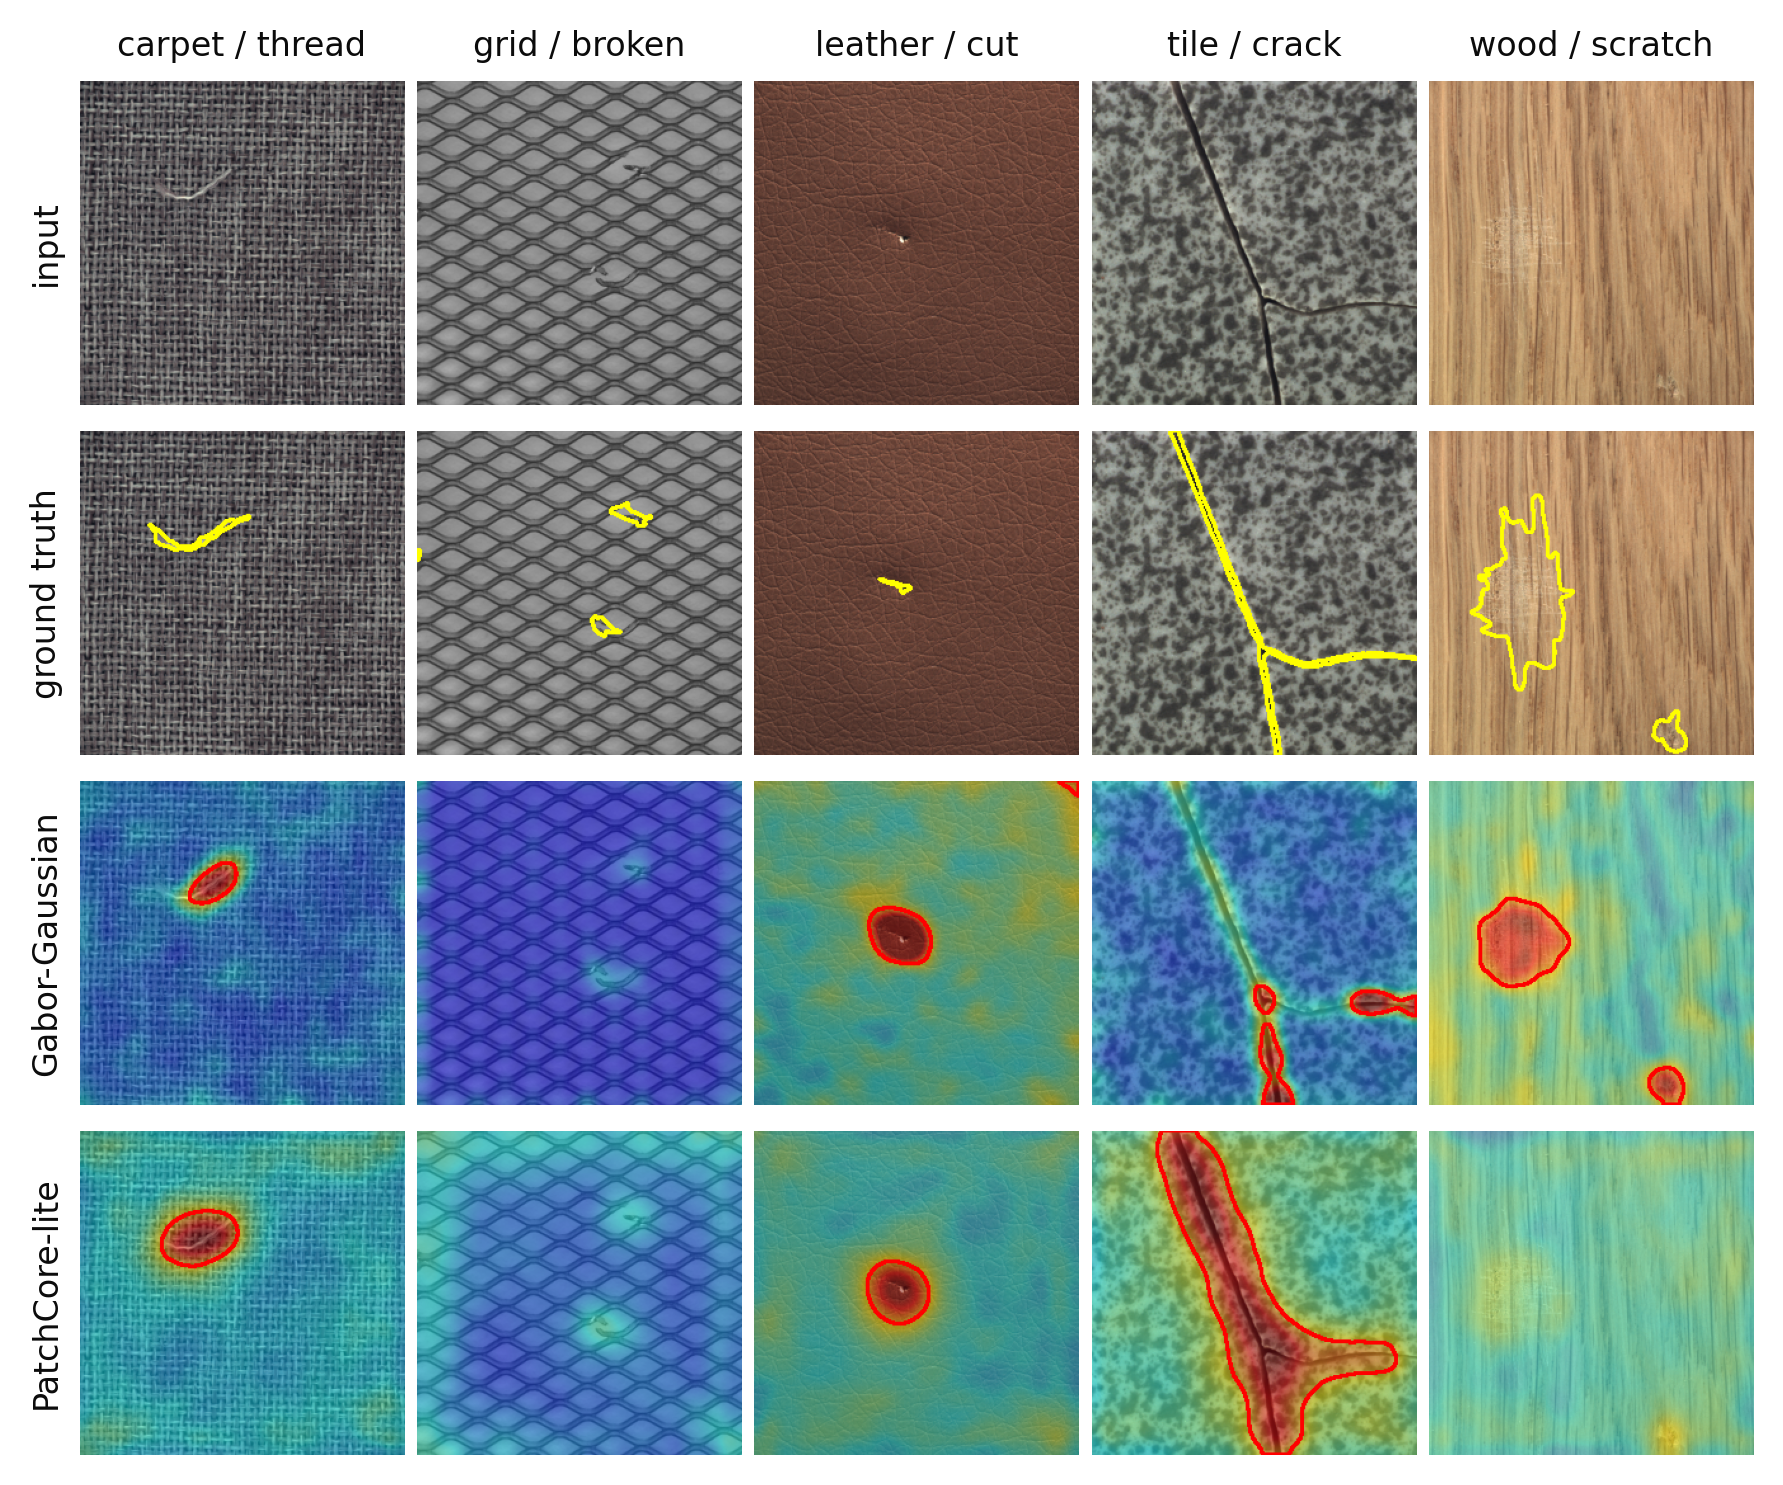
\includegraphics[width=\columnwidth]{fig_qualitative.png}
\caption{Anomaly maps of the station (Gabor--Gaussian) and edge (PatchCore-lite) models ($k=10$). Yellow: ground truth; red: regions above the label-free threshold.}
\label{fig:qual}
\end{figure}

\subsection{Label-Free Thresholds}\label{sec:res-threshold}
With the LOO threshold (\ref{eq:tau}), PatchCore-lite at $k=10$ and $m=0.1$ produces 3.4\,\% false alarms on good test images at 71.8\,\% defect recall (F1 0.753, mean of five textures and three draws). Without margin, recall rises to 78.8\,\% but false alarms to 24.5\,\%; $m=0.2$ removes false alarms entirely at 65.3\,\% recall, so $m$ is a single, interpretable knob between nuisance stops and escapes. Results are similar for $k=5$ and $20$ (F1 0.755 and 0.754). Grid is the exception: its LOO threshold is so conservative that almost no defect is flagged (F1 0.023); on the other four textures PatchCore-lite reaches F1 0.935 at 4.3\,\% false alarms and 89.4\,\% recall. The station model's LOO threshold is far less reliable (28.2\,\% false alarms at $k=10$, $m=0.1$), dominated by leather (95.8\,\%) and carpet (38.1\,\%), where ten LOO scores underestimate the range of normal scores. The station threshold is therefore best used to \emph{define} an uncertainty band rather than to issue final verdicts near the boundary.
